% !TeX root = main.tex
\documentclass{beamer}

% ==================================================================
% Packages & Setup
% ==================================================================
\usepackage[utf8]{inputenc}
\usepackage{amsmath}
\usepackage{amssymb}
\usepackage{graphicx}
\usefonttheme[onlymath]{serif}
\usepackage{algorithm}
\usepackage{algpseudocode}
\usepackage{xcolor}
\setbeamertemplate{bibliography item}[text]

% --- Theme Setup ---
\usetheme{Madrid}

% --- Auto-Outline at beginning of each section ---
\AtBeginSection[]{
    \begin{frame}
        \frametitle{Outline}
        \tableofcontents[currentsection, hideothersubsections, sectionstyle=show/shaded]
    \end{frame}
}

% ==================================================================
% Title Information
% ==================================================================
\title{Extending L* algorithm to Learn Syntactic Monoids}
\author{Haotian Zhang}
\date{\today}

\begin{document}

% ------------------------------------------------------------------
% Title Page
% ------------------------------------------------------------------
\frame{\titlepage}

% ------------------------------------------------------------------
% Main Outline
% ------------------------------------------------------------------
\begin{frame}
    \frametitle{Outline}
    \tableofcontents
\end{frame}


% ==================================================================
% Section 1: L* Algorithm
% ==================================================================
\section{L* algorithm}

% ------------------------------------------------------------------
% Frame: Concept of L* (Membership & Equivalence Queries)
% ------------------------------------------------------------------
\begin{frame}{L* algorithm - Learning Minimal DFA}
    \begin{block}{L* algorithm -- Learning a minimal DFA}
        For an unknown regular language $U \subseteq \Sigma^*$, find $U$'s expression using two types of queries:\cite{angluin87}
        \begin{itemize}
            \item \textbf{Membership query:} For a word $w \in \Sigma^*$, is $w \in U$?
            \item \textbf{Equivalence query:} For a DFA $\mathcal{A}$, is $L(\mathcal{A}) = U$? If the answer is no, then we can obtain a counterexample. 
        \end{itemize}
    \end{block}
    
    \begin{columns}
        \begin{column}{0.6\textwidth} 
            \centering
            % 
            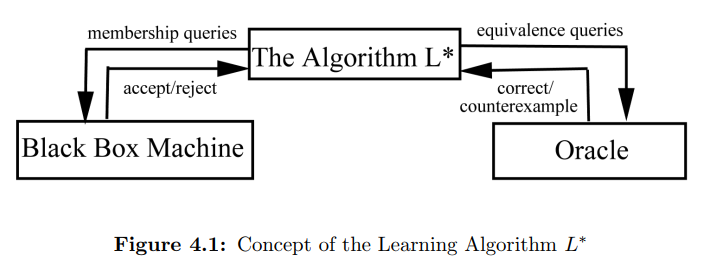
\includegraphics[width=\textwidth]{L-star-concept.png} 
        \end{column}
    \end{columns}
\end{frame}

% ------------------------------------------------------------------
% Frame: Observation Table Definition
% ------------------------------------------------------------------
\begin{frame}{L* algorithm - Observation Table }
    \begin{columns}[T]
        % --- Left Column: Definitions ---
        \begin{column}{0.6\textwidth}
            \begin{itemize}
                \item $U$ : Unknown regular language. 
                \item $\Sigma$ : Alphabet, in example it is $\{a,b\}$
                \item $I$ : Set of test states
                \item $S$ : Set of suffixes
                \item $T$: $(I \cup I \cdot \Sigma \times S) \to \{0,1\}$
                \item $OT$ : {\small Observation table, a 3-tuple } $(I,S,T)$
                \item $\text{row}(i)$: A function $\text{row} \colon I \times S \to \{0,1\}$ defined by
                $\text{row}(i)(s) = T(i,s)$.
            \end{itemize}
        \end{column}

        % --- Right Column: Example Table ---
        \begin{column}{0.6\textwidth}
            \centering
            \begin{tabular}{cc|c|c}
                &   & \multicolumn{2}{c}{$S$} \\ 
                \multicolumn{2}{c|}{} & $\epsilon$ & a \\ \hline
                & $\epsilon$ & 1 & 0 \\
                {$I$}& a          & 0 & 1 \\
                & b          & 0 & 0 \\\hline
                & aa& 1& 0 \\
                {$I\cdot \Sigma$}        & ab& 0&0\\
                & ba         & 0 & 0 \\
                & bb         & 1 & 0 \\ 
            \end{tabular}
            \par \vspace{0.2cm} 
            {\footnotesize $L = (aa + a^* b a^* b)^*$}
        \end{column}
    \end{columns}
\end{frame}

% ------------------------------------------------------------------
% Frame: Closed & Separable Definitions
% ------------------------------------------------------------------
\begin{frame}{L* algorithm - Closed \&  Separable}
    \textbf{Suffix-equivalent for $u, v \in \Sigma^{*}$: }
    $$
        u \equiv_{S} v
        \Leftrightarrow
        \text{row}(u) = \text{row}(v)
        \Leftrightarrow
        \forall s \in S,\ \text{row}(u)(s) = \text{row}(v)(s)
    $$
    \textbf{\small Separable}: \small no two distinct words in $I$ are \textbf{Suffix-equivalent}. 

    \textbf{Closed: }
    $$
        \forall i \in I , a \in \Sigma, \exists i^{\prime} \in I.ia \equiv_{S} i^{\prime}
    $$
    \centering
    \begin{tabular}{cc|c|c}
        &   & \multicolumn{2}{c}{$S$} \\ 
        \multicolumn{2}{c|}{} & $\epsilon$ & a \\ \hline
        & $\epsilon$ & 1 & 0 \\
        {$I$}& a          & 0 & 1 \\
        & b          & 0 & 0 \\ \hline
        
        & aa& 1& 0 \\
        {$I \cdot \Sigma$}& ab& 0&0\\
        & ba         & 0 & 0 \\
        & bb         & 1 & 0 \\  
    \end{tabular}
\end{frame}

% ------------------------------------------------------------------
% Frame: Acceptor Definition
% ------------------------------------------------------------------
\begin{frame}{Acceptor}
    The \textbf{Acceptor} of $(I,P,S,T)$ is a 5-tuple $\mathcal{M} = (Q,\Sigma,\delta,q_0,F)$:
    \begin{itemize}
        \item $Q = \{\text{row}(i) \mid i \in I\}$
        \item $q_0 = \text{row}(\epsilon) \in Q$
        \item $F = \{\text{row}(i) \in Q \mid \text{row}(i)(\epsilon) = 1\}$
        \item $\delta \colon Q \times \Sigma \to Q$ is the transition function.
    \end{itemize}
    \begin{block}{Construction of transition function}
        For $q \in Q, a \in \Sigma$, if $q = \text{row}(i)$ ($i \in I$) and we have
        $ia \equiv_{S} i'$, $i' \in I$, then:
        \[
            \delta(q,a) = \text{row}(i')
        \]
        The transition function $\delta$ is extended to $\delta^{*} \colon Q \times \Sigma^{*} \to Q$:
        \[
            \delta^{*}(q,w) = 
            \begin{cases}
                q & \text{if } w = \epsilon \\
                \delta(\delta^*(q,w'),a) & \text{if } w = w'a, a \in \Sigma
            \end{cases}
        \]
    \end{block}
\end{frame}

% ------------------------------------------------------------------
% Frame: Process Step 1 & 2 (Table Expansion)
% ------------------------------------------------------------------
\begin{frame}{L* algorithm - Algorithmic Process}
    1. $I:= S := \{\epsilon\}$\\
    2. If $OT$ is not closed but separable, use \textbf{membership queries} to find a
    $w^{\prime} \in I \cdot \Sigma$ such that
    $\text{row}(w^{\prime}) \ne \text{row}(w)$ for every $w \in I$.
    Add $w^{\prime}$ to $I$ and expand $I \cdot \Sigma$.
    Repeat this operation until $OT$ is separable and closed.\\
    
    \begin{columns}[T]
        % --- Left Column: Not Closed Example ---
        \begin{column}{0.45\textwidth} 
            \centering
            \begin{tabular}{cc|c|c}
                &   & \multicolumn{2}{c}{$S$} \\ 
                \multicolumn{2}{c|}{} & $\epsilon$ & a \\ \hline
                & $\epsilon$ & 1 & 0 \\
                {$I$}& a          & 0 & 1 \\ \hline
                 & \textcolor{red}{b}          & 0 & 0 \\
                {$I \cdot \Sigma$}           & aa& 1& 0 \\
                & ab& 0&0\\ 
                \multicolumn{4}{c}{} \\[-0.8em] 
                \multicolumn{4}{c}{\footnotesize Not closed}
            \end{tabular}
        \end{column}
    
        % --- Right Column: Closed Example ---
        \begin{column}{0.45\textwidth} 
            \centering
            \begin{tabular}{cc|c|c}
                &   & \multicolumn{2}{c}{$S$} \\ 
                \multicolumn{2}{c|}{} & $\epsilon$ & a \\ \hline
                & $\epsilon$ & 1 & 0 \\
                {$I$}& a          & 0 & 1 \\
                & \textcolor{red}{b}          & 0 & 0 \\\hline
                & aa& 1& 0 \\
                {$I\cdot \Sigma$}        & ab& 0&0\\
                & \textcolor{red}{ba}         & 0 & 0 \\
                & \textcolor{red}{bb}           & 1 & 0 \\ 
                \multicolumn{4}{c}{} \\[-0.8em] 
                \multicolumn{4}{c}{\footnotesize Closed}
            \end{tabular}
        \end{column}
    \end{columns}
\end{frame}


% ------------------------------------------------------------------
% Frame: Process Step 3-6 (Equivalence Query & Loop)
% ------------------------------------------------------------------
\begin{frame}{L* algorithm - Algorithmic Process}
    3. We can get an \textbf{Acceptor} (hypothesis automaton) and ask an \textbf{equivalence query} for it. \\
    4. If the answer is yes, algorithm terminates and \textbf{Acceptor} is the answer. \\
    5. If the answer is no, find a counterexample $w$ in $O(log|w|)$\cite{rivest1993inference}. Properly find the most precise suffix and add it to $S$. Now $OT$ must not be closed. \\
    6. Return to 2. 
    
    \begin{columns}
        \begin{column}{0.4\textwidth} 
            \centering
            % 
            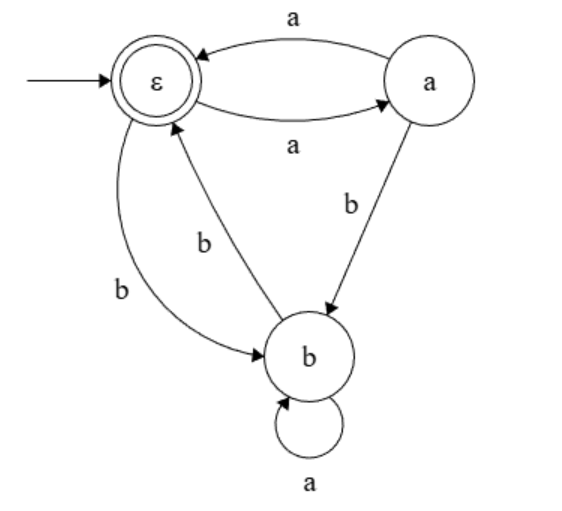
\includegraphics[width=\textwidth]{automaton.png} 
             \par \vspace{0.2cm} 
            {\footnotesize $L = (aa + a^* b a^* b)^*$}
        \end{column}
    \end{columns}
\end{frame}


% ------------------------------------------------------------------
% Frame: Process Step Summary
% ------------------------------------------------------------------
\begin{frame}{L* algorithm - Algorithmic Process}
    
    \begin{columns}
        \begin{column}{1.0\textwidth}
            \centering
            % 
            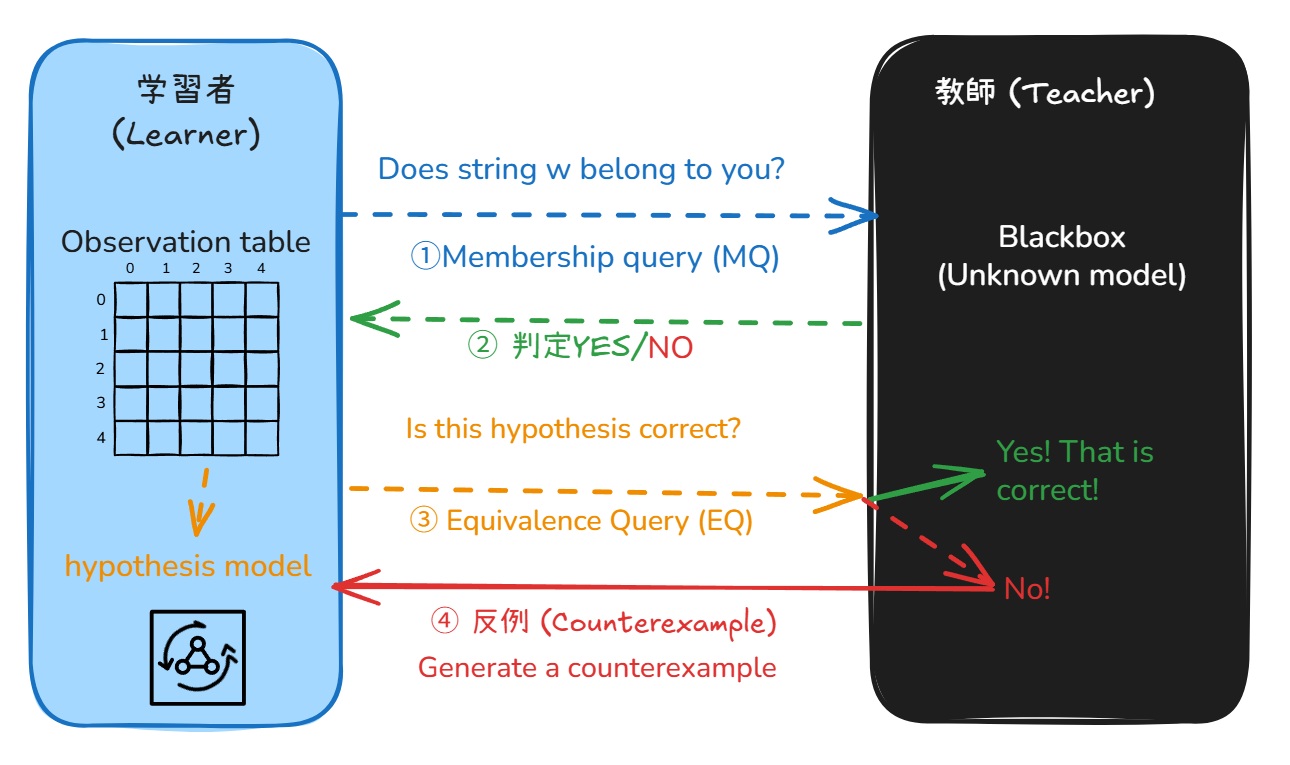
\includegraphics[width=\textwidth]{algorithm_process.png} 
             \par \vspace{0.2cm} 
        \end{column}
    \end{columns}
\end{frame}


% ==================================================================
% Section 2: Minimal DFA vs. Syntactic Monoid
% ==================================================================
\section{Minimal DFA vs. Syntactic Monoid}

% ------------------------------------------------------------------
% Frame: Definition of Minimal DFA
% ------------------------------------------------------------------
\begin{frame}{Minimal DFA}

    Let $L$ be a regular language.
    \begin{block}{Minimal DFA of L, $A_L$}
        {\small The DFA with the minimum number of states that recognizes $L$.}
        \begin{itemize}
            \item The set of states is the quotient set by the Myhill-Nerode (right) congruence:
            $$ w \equiv_{L} w' \iff \forall v \in \Sigma^*. (wv \in L \iff w'v \in L) $$
            The state set is $\Sigma^* / \equiv_L$.
        \end{itemize}
    \end{block}
\end{frame}

% ------------------------------------------------------------------
% Frame: Definition of Syntactic Monoid
% ------------------------------------------------------------------
\begin{frame}{Syntactic Monoid}
    Let $L$ be a regular language.
    \begin{block}{Syntactic Monoid of L, $M_L$}
        The monoid with the minimum order that recognizes $L$.
        \begin{itemize}
            \item The underlying set is the quotient set by the syntactic congruence:
            $$ w \cong_{L} w' \iff \forall u, v \in \Sigma^*. (uwv \in L \iff uw'v \in L) $$
            The set is $\Sigma^* / \cong_L$.
        \end{itemize}
    \end{block}
\end{frame}

% ------------------------------------------------------------------
% Frame: Comparison Example (DFA vs Monoid)
% ------------------------------------------------------------------
\begin{frame}{Minimal DFA vs. Syntactic Monoid}
    \textbf{Example:} Let $L = (ab)^* \subseteq \{a, b\}^*$.
    \vspace{-0.4em} 
    \begin{columns}
        % --- Left: Minimal DFA ---
        \begin{column}{0.48\textwidth} 
            \centering
            \textbf{Minimal DFA $A_L$} 
            % 
            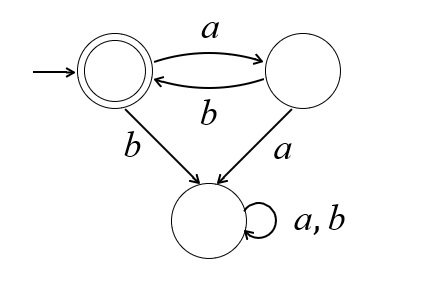
\includegraphics[width=\textwidth]{1.png} 
        \end{column}
    
        % --- Right: Syntactic Monoid ---
        \begin{column}{0.48\textwidth} 
            \centering
            \textbf{Syntactic Monoid $M_L$} 
            (Right Cayley Graph) 
            % 
            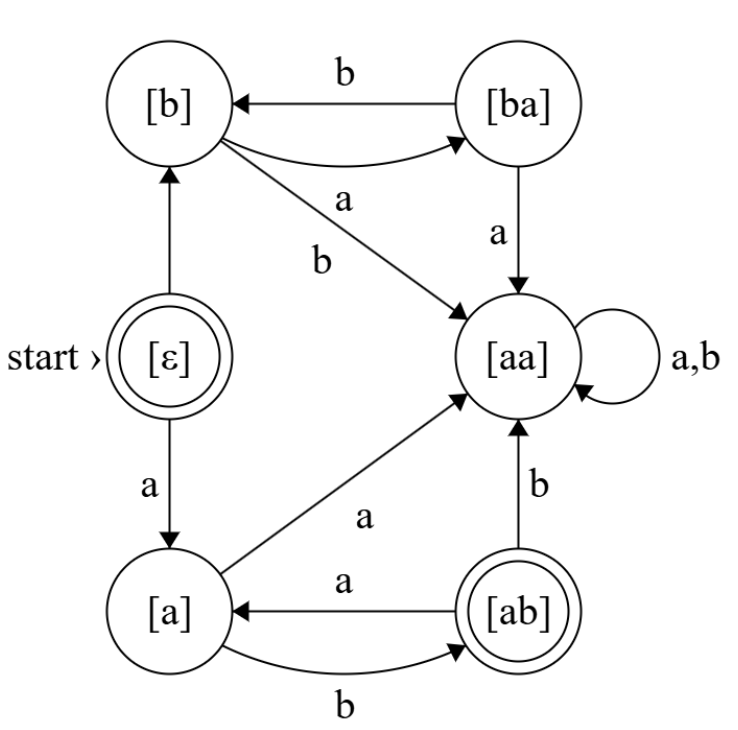
\includegraphics[width=\textwidth]{2.png} 
        \end{column}
    \end{columns}
\end{frame}

% ------------------------------------------------------------------
% Frame: Motivation
% ------------------------------------------------------------------
\begin{frame}{Motivation}
    $|M_L| = M$, $|A_L| = n$ and $|\Sigma| = k$.
    \begin{block}{Properties of Syntactic Monoids}
        \begin{itemize}
            \item \small In general, $M \ge n$. 
            \item \small Generally the upper bound of $M$ is $n^n$.
            \item \small The way to construct the syntactic monoid from the minimal DFA, the time comlexity is $O(kMn)$ \cite{froidure1997algorithms}.
            \item \small  Many language properties have direct algebraic characterizations through syntactic monoids, e.g.,
star-freeness, commutativity, and being a group language.
        \end{itemize}
    \end{block}
\end{frame}


% ------------------------------------------------------------------
% Frame: Motivation
% ------------------------------------------------------------------
\begin{frame}{Motivation}
    \begin{block}{Example - Star-freeness}
        \begin{itemize}
        \item Star-free languages are described using union,
        concatenation, and complement, without the Kleene star.
        \item For example, $(ab)^*$ is star-free:
        \[
        (ab)^*=
        \overline{
        b\Sigma^*\cup\Sigma^*a
        \cup\Sigma^*(aa\cup bb)\Sigma^*
        },
        \qquad \Sigma^*=\overline{\emptyset}.
        \]
        \item Minimal DFA characterization:
        \[
        L\text{ is star-free}
        \Longleftrightarrow A_L\text{ is permutation-free}.
        \quad \cite{thomas2005applied}
        \]
        Deciding this from a DFA is PSPACE-complete.

        \item Syntactic monoid characterization:
        \[ \small
        \begin{aligned}
        L \text{ is star-free}
        \Leftrightarrow M_L \text{ is aperiodic} 
        \Leftrightarrow
        \forall m\in M_L,\ \exists n\geq 1:
        m^n = m^{n+1}.
        \end{aligned}
        \quad \cite{SCHUTZENBERGER1965190}
        \]
        Deciding this is in $O(M^2)$.
    \end{itemize}
    \end{block}
\end{frame}

% ------------------------------------------------------------------
% Frame: Motivation
% ------------------------------------------------------------------
\begin{frame}{Motivation}
    \begin{block}{Research Question}
        \begin{itemize}
            \item Suppose that an unknown regular language $L$
            is accessible only through membership and equivalence queries.

            \item The traditional approach:
            \[
            \text{Queries}
            \longrightarrow A_L
            \longrightarrow M_L
            \longrightarrow \text{Property checking}.
            \]

            \item Can we instead refine the language behavior and its
            algebraic structure together during active learning?
            \[
            \text{Queries}
            \longrightarrow M_L
            \longrightarrow \text{Property checking}.
            \]
        \end{itemize}
    \end{block}
\end{frame}

% ------------------------------------------------------------------
% Frame: Motivation
% ------------------------------------------------------------------
\begin{frame}{Motivation}
   
    \begin{alertblock}{Our Goal}
        \begin{itemize}
            \item Extend the L* algorithm to actively learn the syntactic monoid rather than constructing it only as a post-processing step.
            \begin{itemize}
                \item Design new algorithm based on 2 types of queries.
                \item Prove the correctness.
                \item Analyze the complexity.
            \end{itemize}
            \item Expected benefits: Investigate whether this integrated approach can improve efficiency in properties checking for languages. 
        \end{itemize}
    \end{alertblock}
\end{frame}
% ==================================================================
% Section 3: Idea of Learning Syntactic Monoid
% ==================================================================
\section{Idea of Learning Syntactic Monoid}


% ------------------------------------------------------------------
% Frame: Extended Observation Table (4-tuple)
% ------------------------------------------------------------------
\begin{frame}{Summary of Ideas}
    \begin{itemize}
        \item Extend the observation table to examine both
        left and right contexts.

        \item Construct a hypothesis acceptor intended to represent
        the Right Cayley Graph of the syntactic monoid.

        \item Refine the observation table using membership and
        equivalence queries.
    \end{itemize}
\end{frame}


\begin{frame}{Summary of Ideas}
    \begin{alertblock}{Why Are New Properties Needed?}
        \begin{itemize}
            \item \textbf{Right Consistency:}
            Closedness alone does not guarantee that
            status-equivalent words remain equivalent after
            right multiplication:
            \[
                u \equiv_{\mathrm{status}} v
                \not\Rightarrow
                ua \equiv_{\mathrm{status}} va.
            \]
            Thus, the observed equivalence may not correctly
            represent the right action.

            \item \textbf{Monoid Consistency:}
            Even if the hypothesis recognizes the correct language,
            \[
                L(\mathcal{M})=U,
            \]
            it may still merge words from different syntactic
            congruence classes and therefore fail to be the
            Right Cayley Graph of the syntactic monoid.
        \end{itemize}
    \end{alertblock}
\end{frame}

% ------------------------------------------------------------------
% Frame: Extended Observation Table (4-tuple)
% ------------------------------------------------------------------
\begin{frame}{Idea - Terminology}
    Define a function $\chi: \Sigma^* \to \{0,1\}$ using membership query. 
    \[
    \chi(w) = \begin{cases} 
        1, & \text{if } w \in U \\ 
        0, & \text{if } w \notin U 
    \end{cases}
    \]
    \begin{itemize}
        \item $U$ : Unknown regular language
        \item $\Sigma$ : Alphabet
        \item \textbf{\color{red}{$P$}} : Set of prefixes
        \item $S$ : Set of suffixes
        \item $I$ : Set of test states
        \item \textbf{\color{red}{$T$}}: $P\times (I \cup I \cdot \Sigma) \times S \to \{0,1\}$
        \item \textbf{\color{red}{$OT$}} : {\small Observation table. Actually it is a 4-tuple} $(P,I,S,T)$
        \item \textbf{\color{red}{$row_{P,S}(i)$}}: $(\chi(p\cdot i \cdot s))_{(p,s) \in P \times S}$. Use $row(i)$ to express $row_{P,S}(i)$ if not specified.
        \item \textbf{\color{red}{$row_{S}(i)$}}: $(\chi(\epsilon \cdot i \cdot s))_{s \in S}$
    \end{itemize}    
\end{frame}


% ------------------------------------------------------------------
% Frame: Status-equivalent & Closed
% ------------------------------------------------------------------
\begin{frame}{Idea - Closed \& Separable}
    \textbf{Status-equivalent for $i, i^{\prime}\in \Sigma^{*}$: }
    $$
        i \equiv_{status} i^{\prime} \Leftrightarrow  \forall p \in P,s \in S. \text{row}(i)(p,s) = \text{row}(i^{\prime})(p,s)
    $$
    \textbf{Separable}: no two distinct words in $I$ are \textbf{Status-equivalent}. 
    
    \textbf{Closed: }
    $$
        \forall i^{\prime} \in I \cdot \Sigma,  \exists i \in I.(i \equiv_{status} i^{\prime}) 
    $$
\end{frame}

% ------------------------------------------------------------------
% Frame: Acceptor Definition
% ------------------------------------------------------------------
\begin{frame}{Acceptor}
    The \textbf{Acceptor} of $(I,P,S,T)$ is a 5-tuple
    $\mathcal{M}=(Q,\Sigma,\delta,q_0,F)$:
    \begin{itemize}
        \item $Q=\{\text{row}(i)\mid i\in I\}$
        \item $q_0=\text{row}(\epsilon)\in Q$
        \item $F=\{\text{row}(i)\in Q \mid \text{row}(i)(\epsilon,\epsilon)=1\}$
        \item $\delta\colon Q\times\Sigma\to Q$ is the transition function.
    \end{itemize}

    \begin{block}{Construction of the transition function}
        For $q\in Q$ and $a\in\Sigma$, if
        $q=\text{row}(i)$ for some $i\in I$, and
        $ia\equiv_{status}i'$ for some $i'\in I$, then
        \[
            \delta(q,a)=\text{row}(i').
        \]

        The transition function $\delta$ is extended to
        $\delta^*\colon Q\times\Sigma^*\to Q$:
        \[
            \delta^*(q,w)=
            \begin{cases}
                q & \text{if }w=\epsilon,\\
                \delta(\delta^*(q,w'),a)
                & \text{if }w=w'a,\ a\in\Sigma.
            \end{cases}
        \]
    \end{block}
\end{frame}

% ------------------------------------------------------------------
% Frame: Right Consistency
% ------------------------------------------------------------------
\begin{frame}{Idea - Suffix Equivalent and Right Consistency}
    \textbf{Suffix-equivalent for $i, i^{\prime}\in \Sigma^{*}$: }
    $$
        i \equiv_{S} i^{\prime} \Leftrightarrow  \forall s \in S. \text{row}(i)(\epsilon,s) = \text{row}(i^{\prime})(\epsilon,s)
    $$

    \textbf{Right Consistency: }
    $$
        \forall i,i^{\prime} \in I,a \in \Sigma. i \equiv_{S} i^{\prime} \Leftrightarrow  ia \equiv_{S} i^{\prime}a
    $$
\end{frame}

% ------------------------------------------------------------------
% Frame: Necessity of Right Consistency
% ------------------------------------------------------------------
\begin{frame}{Necessity of Right Consistency}
    \textbf{Problem:} Two status-equivalent words may not go to the same state after right multiplication, which means that the acceptor may not correctly represent the right action.
    \begin{columns}[T]
        \begin{column}{0.55\textwidth}
            \centering
            \textbf{Observation Table}

            % 在这里粘贴只扩展 P 的 observation table
            \begin{table}
                \centering
                \resizebox{0.82\textwidth}{!}{
                    \begin{tabular}{cc|ccccc}
                        & & \multicolumn{5}{c}{$P\times S$} \\
                        & $i$
                        & $(\epsilon,\epsilon)$
                        & $(a,\epsilon)$
                        & $(b,\epsilon)$
                        & $(ab,\epsilon)$
                        & $(bb,\epsilon)$ \\ \hline

                        & $\epsilon$ & 1 & 0 & 0 & 0 & 0 \\
                        & $a$        & 0 & 1 & 0 & 0 & 0 \\
                        $I$ & $b$    & 0 & 0 & 0 & 0 & 1 \\
                        & $ab$       & 0 & 0 & 0 & 0 & 0 \\
                        & $bb$       & 0 & 0 & 1 & 0 & 0 \\ \hline

                        & $aa$       & 1 & 0 & 0 & 0 & 0 \\
                        & $ba$       & 0 & 0 & 0 & 0 & 0 \\
                        $I\cdot\Sigma$ & $aba$ & 0 & 0 & 0 & 0 & 0 \\
                        & $abb$      & 0 & 0 & 0 & 0 & 0 \\
                        & $bba$      & 0 & 0 & 0 & 0 & 0 \\
                        & $bbb$      & 1 & 0 & 0 & 0 & 0
                    \end{tabular}
                }
            \end{table}
            \vspace{0.2cm}
                The table is closed and separable, but not right consistent.
        \end{column}

        \begin{column}{0.43\textwidth}
            \centering
            \textbf{Hypothesis DFA}

            \vspace{0.2cm}

            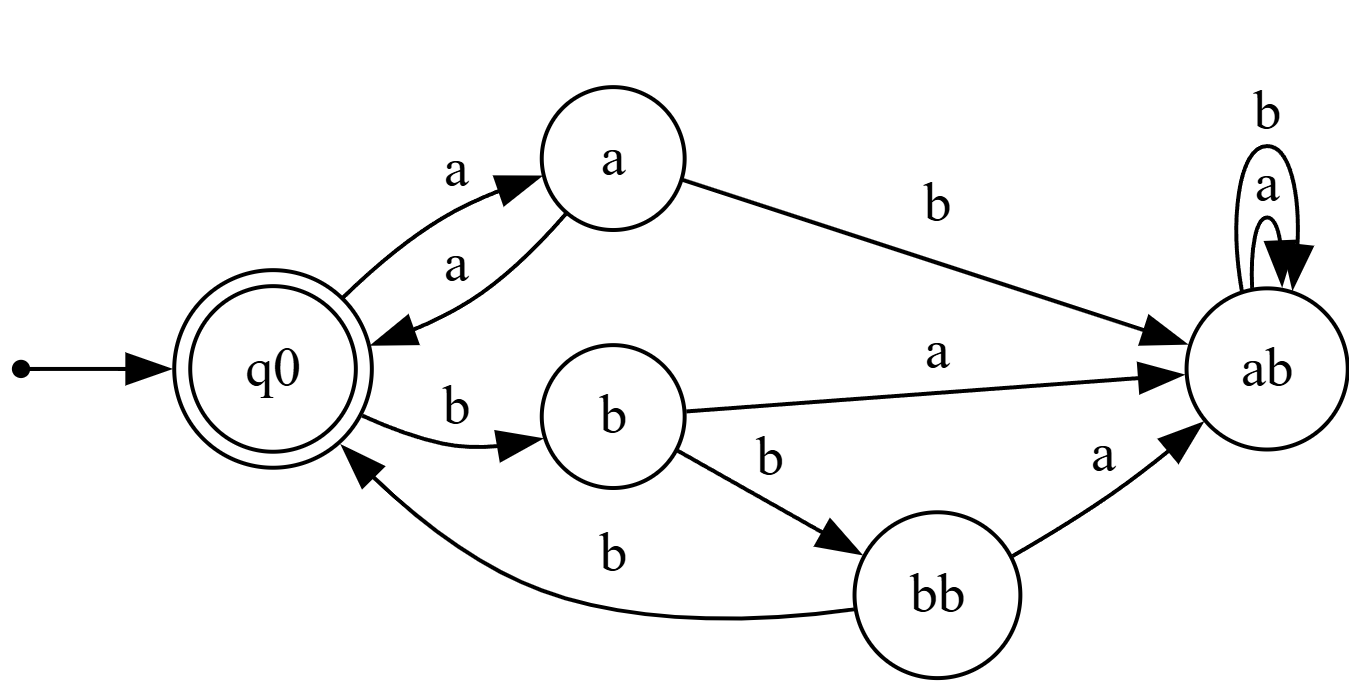
\includegraphics[width=\textwidth]{wrongDFA.png}

            \vspace{0.2cm}
            \[
                L(\mathcal{A})= U = (aa|bbb)^*.
            \]
            The hypothesis is a correct minimal DFA.

        \end{column}
    \end{columns}
\end{frame}

% ==================================================================
% Slide: Necessity of Right Consistency
% ==================================================================
\begin{frame}{Necessity of Right Consistency}
    \begin{block}{Right Consistency Violation}
    Since $S=\{\epsilon\}$,
    \[
    \text{row}_S(a)=\text{row}_S(ab)=(0).
    \]
    However, after right multiplication by $a$,
    \[
    \text{row}_S(aa)=(1)
    \neq
    (0)=\text{row}_S(aba).
    \]
\end{block}

\begin{alertblock}{Repair}
    Add the distinguishing suffix $a$ to $S$:
    \[
    S\leftarrow S\cup\{a\}.
    \]
    Then $\text{row}_S(a)\neq\text{row}_S(ab)$, clearly $\text{row}(a)\neq\text{row}(ab)$, therefore the table is not closed and we can add $ab$ into $I$ to make the table closed again.
\end{alertblock}
\end{frame}

% ==================================================================
% Slide: Right Consistency and the Acceptor
% ==================================================================

\begin{frame}{Path Representative Function}
    \begin{block}{Definition of Representative Function}
        Assume that the observation table is closed.
        Define the Path representative function $\rho:\Sigma^*\to I$ recursively as follows:
        \[
        \rho(\epsilon)=\epsilon,
        \]
        and for every $x = ya(x,y\in\Sigma^*, a\in\Sigma)$ and $\rho(y) = i (i\in I)$. Then because of closedness:
        \[
        \exists u \in I. ia \equiv_{status} u.
        \]
        and $\rho(ya) = \rho(x) = u$. 
    \end{block}

    \begin{alertblock}{Intuition}
        If $\delta^*(q_0,w) = q$ for string $w$, because of the definiton of acceptor, there is a path representative $i \in I$ such that $\delta^*(q_0,i) = q$.
    \end{alertblock}
\end{frame}

% ==================================================================
% Slide: Proposition 2 series
% ==================================================================

\begin{frame}{Proposition 2.2 - 2.3}
    \begin{block}{Assumption}
        All propositions in 2.x series assume that the observation table is closed and right consistent, 
        and $L(\mathcal{M}) = U$(passed the equivalence query). 
    \end{block}

    \begin{block}{Propositions}
        \begin{itemize}
            \item Proposition 2.2:  
            \[
                \forall w \in \Sigma^*, w \equiv_S \rho(w).
            \]
            \item Proposition 2.3: 
             \[
                \forall u,v \in \Sigma^*. u \equiv_S v \Rightarrow (\forall y \in \Sigma^*. uy \in U \iff vy \in U). 
            \]
        \end{itemize}
    \end{block}
\end{frame}

% ==================================================================
% Slide: Proposition 2 series
% ==================================================================

\begin{frame}{Proposition 2.4}
    \begin{block}{Proposition}
        \[
            \forall u,v \in \Sigma^*. u \equiv_{status} v \Rightarrow (\forall a \in \Sigma. ua \equiv_{status} va).
        \]
    \end{block}
    \begin{block}{Proof}
        Assume that $u \equiv_{status} v$, therefore we have:
         \[
            \forall p\in P,s\in S. \chi(p\cdot u \cdot s) = \chi(p\cdot v \cdot s).
        \]
        Thus, for every $p \in P$, $pu \equiv_{S} pv$.
        By Proposition 2.3, for every $z \in \Sigma^*$ we have $puz \in U \iff pvz \in U$.
        So take $z = as$, where $a \in \Sigma$ and $s \in S$, we have $puas \in U \iff pvas \in U$.
        Therefore,
        \[
            ua \equiv_{status} va.
        \]
    \end{block}
\end{frame}

\begin{frame}{Proposition 2.5 - 2.6}
    \begin{block}{Propositions}
       \begin{itemize}
            \item Proposition 2.5:  
            \[
                \forall u \in \Sigma^*, u \equiv_{status} \rho(u).
            \]
            This can be easily proved by induction based on the conclusion in Proposition 2.4.
            \item Proposition 2.6: 
             \[
                \forall u,v \in \Sigma^*. u \equiv_{status} v \iff \delta^*(q_0,u) = \delta^*(q_0,v).
            \]
            Therefore, under the assumption we mentioned, two status-equivalent words must go to the same state. 
        \end{itemize}
    \end{block}
\end{frame}
% ------------------------------------------------------------------
% Frame: Monoid consistency
% ------------------------------------------------------------------
\begin{frame}{Idea - Monoid Consistency}
    The definition of \textbf{monoid consistency} is: 
    $$
		\forall v \in I, t\in I\cdot\Sigma. (t \equiv_{status} v) \Rightarrow \forall i\in I, s\in S, T(i\cdot t \cdot s) = T(i \cdot v \cdot s)
    $$
	We will introduce how to check monoid consistency and why we define like this in the following part.		

\end{frame}

% ==================================================================
% Slide: Proposition 4
% ==================================================================
\begin{frame}{Proposition 4.1 and 4.2 - Monoid Consistency Check}
    Assume that the Acceptor $\mathcal{M}$ passes the equivalence query ($L(\mathcal{M}) = U$), 
    but $\mathcal{M}$ is not the Right Cayley Graph of $U$. 
    
    \begin{block}{Proposition 4.1 - Failure of Monoid Consistency}
        According to the assumption, we must have:
        \[
        \exists v \in I, t \in I \cdot \Sigma. (t \equiv_{status} v) \wedge (t \not\sim_L v)
        \]
    \end{block}

    \begin{block}{Proposition 4.2}
        For such $v$ and $t$, the following is correct:
        \[
         \exists i \in I, s \in S. T(i \cdot t \cdot s) \neq T(i \cdot v \cdot s)
        \]
        In other words:
        \[
        (i \cdot t \cdot s \in U \wedge i \cdot v \cdot s \notin U) \vee (i \cdot t \cdot s \notin U \wedge i \cdot v \cdot s \in U)
        \]
    \end{block}
\end{frame}

% ==================================================================
% Slide: Practical Implementation
% ==================================================================
\begin{frame}{Summary and Implementation}
    If the acceptor passes the equivalence query but fails to form a syntactic monoid:
    \begin{enumerate}
        \item There must exist $t \in I \cdot \Sigma$ and $v \in I$ such that $t \equiv_{status} v$ but $t \not\sim_L v$.
        \item For such $t, v$, there must exist $i \in I, s \in S$ s.t. $T(i \cdot t \cdot s) \neq T(i \cdot v \cdot s)$.
    \end{enumerate}

    \begin{block}{Method to check Monoid Consistency}
        \begin{itemize}
            \item Find $t \in I \cdot \Sigma$ and $v \in I$ such that $t \equiv_{status} v$.
            \item For such $t, v$, find $i \in I$ and $s \in S$ to do the membership query on $i \cdot t \cdot s$ and $i \cdot v \cdot s$.
            \item If $T(i \cdot t \cdot s) \neq T(i \cdot v \cdot s)$, then \textbf{add $i$ into $P$} so that we can distinguish $t$ and $v$ to make the observation table not closed.
        \end{itemize}
    \end{block}
\end{frame}

% ------------------------------------------------------------------
% Frame: Extended Process Flow
% ------------------------------------------------------------------
\begin{frame}{Idea -- Process}
\begin{enumerate}
    \item $I := \{\epsilon\}$, $P:=\{\epsilon\}$, $S:= \{\epsilon\}$
    \item \textbf{Closedness Check}: If $OT$ is not closed, find $i \in I\cdot\Sigma $ with new $\text{row}(i)$, add to $I$. Repeat until closed.
    \item \textbf{Right Consistency Check}: If $OT$ is not right consistent, find $as \in \Sigma\cdot S$, add to $S$. Back to step 2.
    \item \textbf{Equivalence Query}: Construct \textbf{Acceptor} $\mathcal{M}$ and perform query.
    \item \textbf{Decision and Monoid Consistency Check}:
    \begin{itemize}
        \item If Equivalence Query is \textbf{Yes}:
        \begin{itemize}
            \item If \textbf{Monoid Consistency} passes $\rightarrow$ Terminate, return $\mathcal{M}$.
            \item If \textbf{Monoid Consistency} fails $\rightarrow$ Find $i \in I$, add to $P$ (table becomes not closed).
        \end{itemize}
        \item If Equivalence Query is \textbf{No}:
        \begin{itemize}
            \item Find counterexample and add suffix $s$ to $S$ (using Rivest-Schapire).
        \end{itemize}
    \end{itemize}
    \item \textbf{Loop}: Return to Step 2.
\end{enumerate}
\end{frame}

% ==================================================================
% Section 4: Example
% ==================================================================
\section{Example}



% ------------------------------------------------------------------
% Frame: Definition for Rivest-Schapire method function
% ------------------------------------------------------------------

\begin{frame}{Definition for Rivest-Schapire method}

To use Rivest-Schapire method \cite{rivest1993inference}, we define a function $\mathcal{X}$ using membership query. 
    \[
    \mathcal{X}(w) = \begin{cases} 
        1, & \text{if } w \in U \\ 
        0, & \text{if } w \notin U 
    \end{cases}
    \]
\end{frame}

% ------------------------------------------------------------------
% Frame: step01
% ------------------------------------------------------------------

\begin{frame}{Idea -- Example}
$$
U = (ab)^* 
$$ 


\begin{center}
    \begin{tabular}{|cc|c|}
        \multicolumn{2}{c|}{} & $(P\times S)$ \\
        \multicolumn{2}{c|}{} & $(\epsilon,\epsilon)$ \\ \hline
        $I$ & $\epsilon$ & 1 \\ \hline
        $I \cdot \Sigma$ & $a$ & 0 \\
        & $b$ & 0 \\ \hline
    \end{tabular}
\end{center}
\end{frame}

% ------------------------------------------------------------------
% Frame: step02
% ------------------------------------------------------------------

\begin{frame}{Idea -- Example}
    \begin{columns}[c] 
        
        % 左侧：放表格
        \begin{column}{0.5\textwidth}
            \centering
            \begin{tabular}{|cc|c|}
                \multicolumn{2}{c|}{} & $(P\times S)$ \\
                \multicolumn{2}{c|}{} & $(\epsilon,\epsilon)$ \\ \hline
                $I$ & $\epsilon$ & 1 \\ 
                    & $a$ & 0 \\\hline
                $I \cdot \Sigma$ & $b$ & 0 \\
                    & $aa$ & 0 \\ 
                    & $ab$ & 1 \\ \hline
            \end{tabular}
        \end{column}

        % 右侧：放图片
        \begin{column}{0.4\textwidth} 
            \centering
            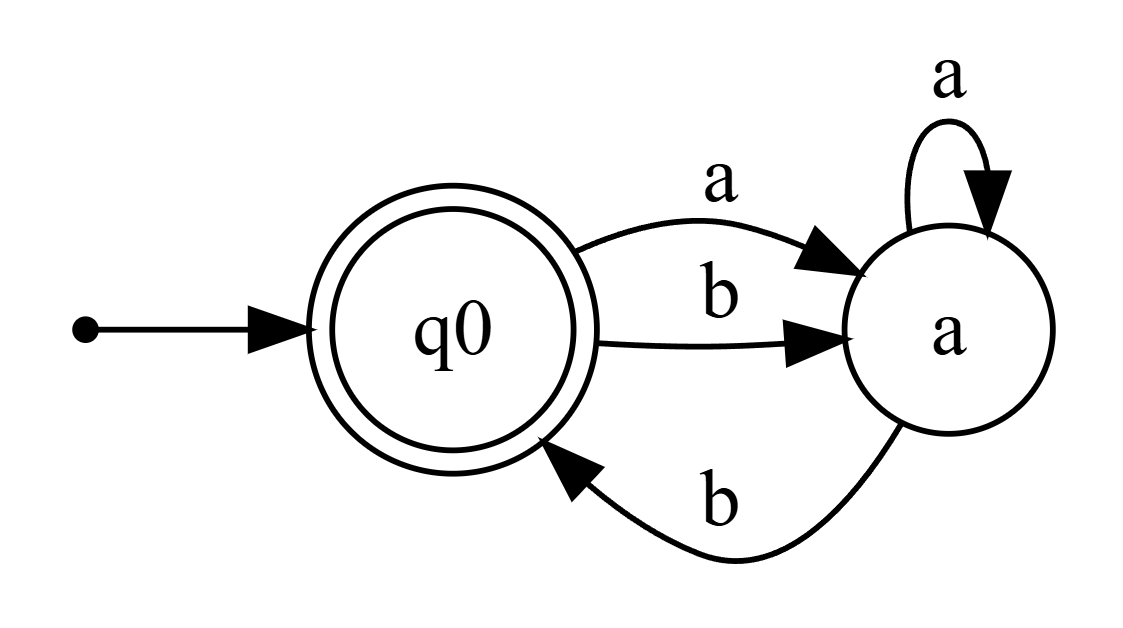
\includegraphics[width=\textwidth]{step_02.png} 
            \par \vspace{0.2cm} 
            {\footnotesize $L(\mathcal{M}) = (\Sigma a^*b)^*$}
        \end{column}
        
    \end{columns}

    \vspace{0.8cm} % 调节这个距离来控制下方留白的大小

    \begin{block}{Counterexample:$bb$ -- Rivest-Schapire method}
    % 下方留出的写字空间
        \begin{enumerate}
            \item $\epsilon \equiv_{status} \epsilon$: $\mathcal{X}(\epsilon \cdot bb) = \mathcal{X}(\epsilon \cdot bb)$
            \item $b \equiv_{status} a$: $\mathcal{X}(b \cdot b) \neq \mathcal{X}(a \cdot b)$
        \end{enumerate}
        \textbf{Conclusion}: The suffix $b$ is the string we are looking for to distinguish the current states.
    \end{block}
\end{frame}


% ------------------------------------------------------------------
% Frame: step03
% ------------------------------------------------------------------

\begin{frame}{Idea -- Example}
\begin{center}
    \begin{tabular}{|cc|c|c|} 
        \multicolumn{2}{c|}{} & \multicolumn{2}{c|}{$(P\times S)$} \\
        \multicolumn{2}{c|}{} & $(\epsilon,\epsilon)$ & $(\epsilon,b)$ \\ \hline
        $I$ & $\epsilon$ & 1 & 0 \\ 
            & $a$ & 0 & 1 \\\hline
        $I \cdot \Sigma$ & $b$ & 0 & 0 \\
            & $aa$ & 0 & 0 \\ 
            & $ab$ & 1 & 0 \\ \hline
    \end{tabular}
\end{center}
\end{frame}

% ------------------------------------------------------------------
% Frame: step04
% ------------------------------------------------------------------
\begin{frame}{Idea -- Example}
% 使用 columns 环境实现左右布局
    \begin{columns}[c] % [c] 表示垂直居中对齐，也可以用 [t] 顶部对齐
        % 左侧：放表格
        \begin{column}{0.5\textwidth}
            \centering
            \begin{tabular}{|cc|c|c|} 
        \multicolumn{2}{c|}{} & \multicolumn{2}{c|}{$(P\times S)$} \\
        \multicolumn{2}{c|}{} & $(\epsilon,\epsilon)$ & $(\epsilon,b)$ \\ \hline
        $I$ & $\epsilon$ & 1 & 0 \\ 
            & $a$ & 0 & 1 \\
            & $b$ & 0 & 0 \\ \hline
        $I \cdot \Sigma$ 
            & $aa$ & 0 & 0 \\ 
            & $ab$ & 1 & 0 \\ 
            & $ba$ & 0 & 0 \\ 
            & $bb$ & 0 & 0 \\ \hline
    \end{tabular}
        \end{column}

        % 右侧：放图片
        \begin{column}{0.4\textwidth} 
            \centering
            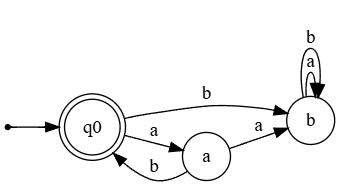
\includegraphics[width=\textwidth]{step_04.png} 
            \par \vspace{0.2cm} 
            {\footnotesize $L(\mathcal{M}) = (ab)^*$}
        \end{column}
    \end{columns}

    \begin{block}{Monoid consistency check}
        \begin{enumerate}
            \item Find status-equivalent pair $(b,aa)$, $(\epsilon,ab)$, $(b,ba)$, $(b,bb)$
            \item $(b,aa)$: 
                \begin{itemize}
                    \item $\text{row}(\epsilon \cdot b) = \text{row}(\epsilon \cdot aa)$
                    \item $\text{row}(a \cdot b) \neq \text{row}(a \cdot aa)$
                    \item $\text{row}(b \cdot b) = \text{row}(b \cdot aa)$
                \end{itemize} 
        \end{enumerate}
        \textbf{Conclusion}: The prefix $a$ is the string we are looking for.
    \end{block}
\end{frame}


% ------------------------------------------------------------------
% Frame: step05
% ------------------------------------------------------------------

\begin{frame}{Idea -- Example}
    \begin{center}
        \begin{tabular}{|cc|c|c|c|c|} 
            \multicolumn{2}{c|}{} & \multicolumn{4}{c|}{$(P\times S)$} \\
            \multicolumn{2}{c|}{} & $(\epsilon,\epsilon)$ & $(\epsilon,b)$ & $(a,\epsilon)$ & $(a,b)$ \\ \hline
            $I$ & $\epsilon$ & 1 & 0 & 0 & 1 \\ 
                & $a$ & 0 & 1 & 0 & 0 \\
                & $b$ & 0 & 0 & 1 & 0 \\ \hline
            $I \cdot \Sigma$ & $aa$ & 0 & 0 & 0 & 0 \\ 
                & $ab$ & 1 & 0 & 0 & 0 \\
                & $ba$ & 0 & 0 & 0 & 1 \\
                & $bb$ & 0 & 0 & 0 & 0 \\ \hline
        \end{tabular}
    \end{center}
\end{frame}

% ------------------------------------------------------------------
% Frame: step06
% ------------------------------------------------------------------

\begin{frame}{Idea -- Example}
    \begin{center}
        \begin{tabular}{|cc|c|c|c|c|} 
    \multicolumn{2}{c|}{} & \multicolumn{4}{c|}{$(P\times S)$} \\
    \multicolumn{2}{c|}{} & $(\epsilon,\epsilon)$ & $(\epsilon,b)$ & $(a,\epsilon)$ & $(a,b)$ \\ \hline
    $I$ & $\epsilon$ & 1 & 0 & 0 & 1 \\ 
        & $a$        & 0 & 1 & 0 & 0 \\
        & $b$        & 0 & 0 & 1 & 0 \\ 
        & $aa$       & 0 & 0 & 0 & 0 \\ \hline
    $I \cdot \Sigma$ & $ab$  & 1 & 0 & 0 & 0 \\
        & $ba$       & 0 & 0 & 0 & 1 \\
        & $bb$       & 0 & 0 & 0 & 0 \\ 
        & $aaa$      & 0 & 0 & 0 & 0 \\ 
        & $aab$      & 0 & 0 & 0 & 0 \\ \hline
\end{tabular}
    \end{center}
\end{frame}

% ------------------------------------------------------------------
% Frame: step07
% ------------------------------------------------------------------

\begin{frame}{Idea -- Example}
    \begin{center}
        \begin{tabular}{|cc|c|c|c|c|} 
    \multicolumn{2}{c|}{} & \multicolumn{4}{c|}{$(P\times S)$} \\
    \multicolumn{2}{c|}{} & $(\epsilon,\epsilon)$ & $(\epsilon,b)$ & $(a,\epsilon)$ & $(a,b)$ \\ \hline
    $I$ & $\epsilon$ & 1 & 0 & 0 & 1 \\ 
        & $a$        & 0 & 1 & 0 & 0 \\
        & $b$        & 0 & 0 & 1 & 0 \\ 
        & $aa$       & 0 & 0 & 0 & 0 \\ 
        & $ab$       & 1 & 0 & 0 & 0 \\ \hline
    $I \cdot \Sigma$ & $ba$  & 0 & 0 & 0 & 1 \\
        & $bb$       & 0 & 0 & 0 & 0 \\ 
        & $aaa$      & 0 & 0 & 0 & 0 \\ 
        & $aab$      & 0 & 0 & 0 & 0 \\ 
        & $aba$      & 0 & 1 & 0 & 0 \\ 
        & $abb$      & 0 & 0 & 0 & 0 \\ \hline
\end{tabular}
    \end{center}
\end{frame}

% ------------------------------------------------------------------
% Frame: step08
% ------------------------------------------------------------------
\begin{frame}{Idea -- Example}
    \begin{columns}[c] 
        % 左侧：放表格
        \begin{column}{0.45\textwidth} % 稍微调大点列宽比例
            \centering
            % 1. 缩小字体 (footnotesize 或 scriptsize)
            \scriptsize 
            % 2. 压缩列间距 (默认是6pt，改为2pt)
            \setlength{\tabcolsep}{2pt} 
            % 3. 稍微压缩行高，让表格别太长
            \renewcommand{\arraystretch}{0.95}

            \begin{tabular}{|cc|c|c|c|c|} 
                \multicolumn{2}{c|}{} & \multicolumn{4}{c|}{$(P\times S)$} \\
                \multicolumn{2}{c|}{} & $(\epsilon,\epsilon)$ & $(\epsilon,b)$ & $(a,\epsilon)$ & $(a,b)$ \\ \hline
                $I$ & $\epsilon$ & 1 & 0 & 0 & 1 \\ 
                    & $a$        & 0 & 1 & 0 & 0 \\
                    & $b$        & 0 & 0 & 1 & 0 \\ 
                    & $aa$       & 0 & 0 & 0 & 0 \\ 
                    & $ab$       & 1 & 0 & 0 & 0 \\ 
                    & $ba$       & 0 & 0 & 0 & 1 \\ \hline
                $I \cdot \Sigma$ & $bb$  & 0 & 0 & 0 & 0 \\
                    & $aaa$      & 0 & 0 & 0 & 0 \\ 
                    & $aab$      & 0 & 0 & 0 & 0 \\ 
                    & $aba$      & 0 & 1 & 0 & 0 \\ 
                    & $abb$      & 0 & 0 & 0 & 0 \\ 
                    & $baa$      & 0 & 0 & 0 & 0 \\ 
                    & $bab$      & 0 & 0 & 1 & 0 \\ \hline
            \end{tabular}
        \end{column}

        % 右侧：放图片
        \begin{column}{0.5\textwidth} 
            \centering
            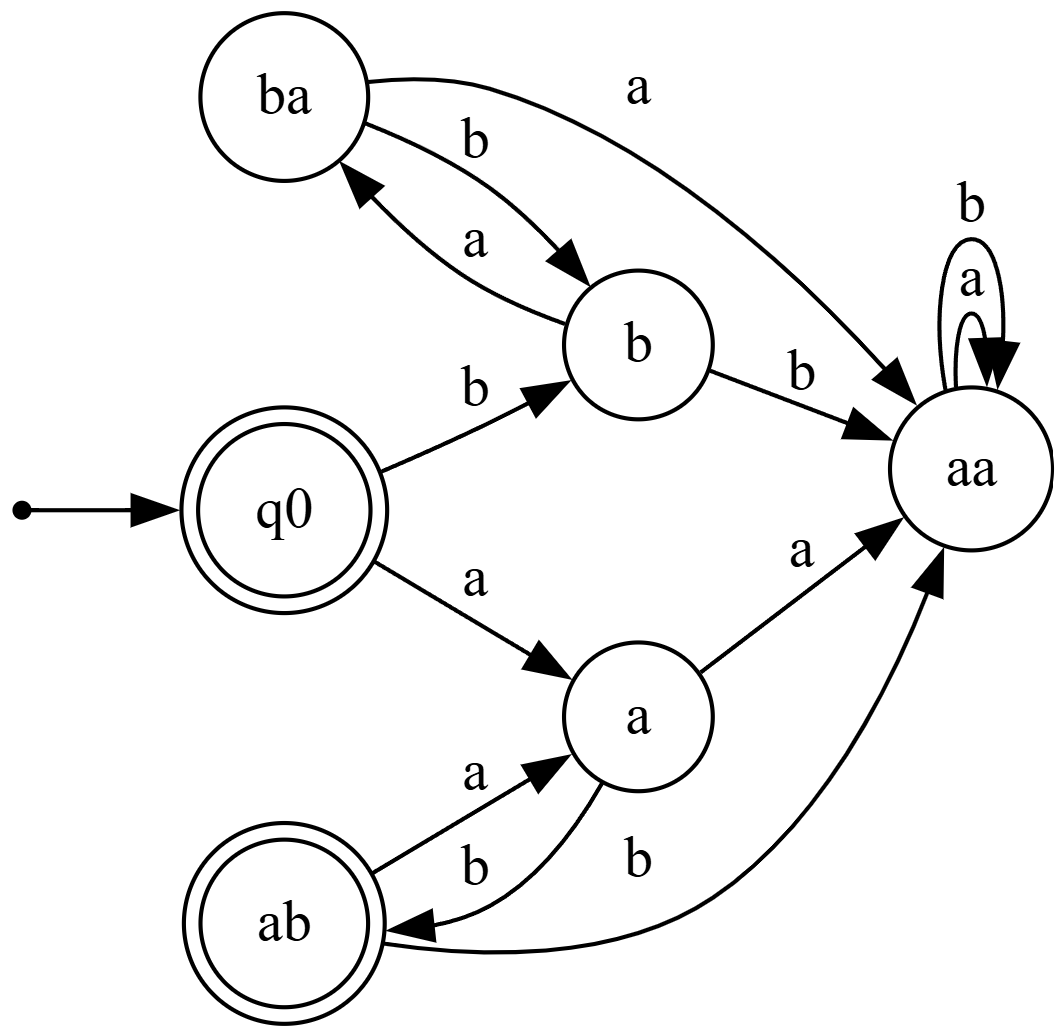
\includegraphics[width=\textwidth]{step_08.png} 
            \par \vspace{0.2cm} 
            {\footnotesize $L(\mathcal{M}) = (ab)^*$}
        \end{column}
    \end{columns}
\end{frame}

% ==================================================================
% Section 5: Future Work
% ==================================================================
\section{Future work}

% ------------------------------------------------------------------
% Frame: Future Tasks
% ------------------------------------------------------------------
\begin{frame}{Summary and Future Work}
    \begin{block}{Summary}
        \begin{itemize}
            \item Extended the L* observation table with both left and right contexts.
            \item Introduced \textbf{Right Consistency} and \textbf{Monoid Consistency}.
            \item Proved that the learned row equivalence correctly supports the right action.
            \item Proved that a language-correct acceptor with no monoid-consistency violation represents the syntactic monoid.
        \end{itemize}
    \end{block}

    \begin{block}{Future Work}
        \begin{itemize}
            \item Analyze the query complexity and time complexity.
            \item Implement the corrected algorithm and compare it with the traditional route:
            \[
                \text{L*}\to A_L\to M_L.
            \]
            \item Reduce redundant rows, contexts, and membership queries during refinement.
        \end{itemize}
    \end{block}
\end{frame}

% ==================================================================
% References
% ==================================================================
\begin{frame}[allowframebreaks] 
    \frametitle{References}
    
    \bibliographystyle{IEEEtran}
    \bibliography{reference} 
\end{frame}

\end{document}